%%%%%%%%%%%%%%%%%%%%%%%%%%%%%%%%%%%%%%%%%%%%%%%%%%%%%%%%%%%%%%%%%%%%%%%%%%%%%%%%
%2345678901234567890123456789012345678901234567890123456789012345678901234567890
%        1         2         3         4         5         6         7         8

\documentclass[letterpaper, 10 pt, conference]{ieeeconf}  % Comment this line out
                                                          % if you need a4paper
%\documentclass[a4paper, 10pt, conference]{ieeeconf}      % Use this line for a4
                                                          % paper

\IEEEoverridecommandlockouts                              % This command is only
                                                          % needed if you want to
                                                          % use the \thanks command
\overrideIEEEmargins
% See the \addtolength command later in the file to balance the column lengths
% on the last page of the document



% The following packages can be found on http:\\www.ctan.org
%\usepackage{graphics} % for pdf, bitmapped graphics files
\usepackage{graphicx} % for png files
\graphicspath{{img/}}
\usepackage{multirow}
%\usepackage[T1]{fontenc}
%\usepackage[utf8]{inputenc}
%\usepackage{epsfig} % for postscript graphics files
%\usepackage{mathptmx} % assumes new font selection scheme installed
%\usepackage{times} % assumes new font selection scheme installed
%\usepackage{amsmath} % assumes amsmath package installed
%\usepackage{amssymb}  % assumes amsmath package installed

\title{\LARGE \bf
Detection of design pattern : A systematic mapping study}

%\author{ \parbox{3 in}{\centering Huibert Kwakernaak*
%         \thanks{*Use the $\backslash$thanks command to put information here}\\
%         Faculty of Electrical Engineering, Mathematics and Computer Science\\
%         University of Twente\\
%         7500 AE Enschede, The Netherlands\\
%         {\tt\small h.kwakernaak@autsubmit.com}}
%         \hspace*{ 0.5 in}
%         \parbox{3 in}{ \centering Pradeep Misra**
%         \thanks{**The footnote marks may be inserted manually}\\
%        Department of Electrical Engineering \\
%         Wright State University\\
%         Dayton, OH 45435, USA\\
%         {\tt\small pmisra@cs.wright.edu}}
%}

\author{Pierre Gerard, Alexandre St-Louis Fortier, Badr Mai and Houari Sahraoui \\
Département IRO \\
Université de Montréal, Montreal, Canada \\
\{gerardpi,stlouial,sahraouh\}@iro.umontreal.ca
% <-this % stops a space
%\thanks{*This work was not supported by any organization}% <-this % stops a space
%\thanks{$^{1}$H. Kwakernaak is with Faculty of Electrical Engineering, Mathematics and Computer Science,
 %       University of Twente, 7500 AE Enschede, The Netherlands
  %      {\tt\small h.kwakernaak at papercept.net}}%
%\thanks{$^{2}$P. Misra is with the Department of Electrical Engineering, Wright State University,
   %     Dayton, OH 45435, USA
    %    {\tt\small p.misra at ieee.org}}%
}


\begin{document}



\maketitle
\thispagestyle{empty}
\pagestyle{empty}


%%%%%%%%%%%%%%%%%%%%%%%%%%%%%%%%%%%%%%%%%%%%%%%%%%%%%%%%%%%%%%%%%%%%%%%%%%%%%%%%
\begin{abstract}

% Place holder
Design patterns are important because they help solving recurring design problems in software engineering. The identification of those patterns can be helpful to maintain and understand the code especially in large systems. Interest in design patterns detection has grown in the last decade.Despite the huge interest given to design patterns detection, there is no reliable or formal method for this matter.
We conducted a systematic mapping study on design patterns detection by querying multiple sources to get articles that are relevant to our study. 403 articles between 2000 and 2015 were considered.
The main purpose of the study is to know which methods and techniques are used to detect design patterns.
The result help us understand how those techniques work and which type of pattern is detected the most.



\end{abstract}


%%%%%%%%%%%%%%%%%%%%%%%%%%%%%%%%%%%%%%%%%%%%%%%%%%%%%%%%%%%%%%%%%%%%%%%%%%%%%%%%
\section{INTRODUCTION}

% Design patterns are a 

Design partterns are best pratices to recurring design problems first proposed
by the Gang of Four in their seminal book.

(Some study author) have been able to show that the presence of design patterns,
if correctly presented, can help developpers better understand a piece of
software [citation needed].
It would therefore be desirable to be able to automatically extract those
design patterns and present them in a digestible format.

Detection of design patterns in software has been a relatively active research
interest of the past decade in software engineering.
Proposed methods of automatic detection aims in part to facilitate the work of
developpers in understanding a piece of software through reverse engineering.

However, design pattern detection tools are still not featured in the typical
programmer toolbox.

No studies have been conducted to analyse the trends of the field.

This paper presents a systematic mapping study on design pattern detection
methods.
It is organized as follows: 
 The first section explains the systematic mapping process
 The second section explains the selection process results
 The third one deals analyses the study results
 The article then continues with the limitations of our study
 It finishes with related work. 

% pourquoi la detection

% pourquoi ce systematic mapping

\section{SYSTEMATIC MAPPING PROCESS}

In this section, we discuss step by step how we conducted our systematic
mapping study.
We have followed the process defined by Petersen et al \cite{c1}. 

\subsection{Research question}

The main goal of this paper is to determine the quantity and trends of research
in design pattern detection and the quality of proposed detection methods.
% TODO: Our classification scheme doesn't really allow us to take any position
% relative to the quality of the methods. At most, it provide a sensible
% evaluation of the field

\begin{itemize}
	\item \textbf{RQ1} : How mature is research on the subject of design pattern detection ?
	\item \textbf{RQ2} : What methods of design pattern detection are used ?
\end{itemize}


\subsection{Data source and queries}

We decided to query only one database, Scopus \cite{c2}, that claims to be the
largest abstract and citation database of peer-reviewed literature.
It indexes the main Computer Science databases : Springer, IEEE, ACM and
others.
The main advantage of using Scopus is that it provides a functionnality to
export the result of a search query on its database.
Some of those exported results would not have been easily obtainable on some
publishers search engines that do not provide an export functionnality.
Consequently, Scopus was used mostly as a Search and Export portal over the
relevant publications, greatly reducing the effort needed to extract the
original articles set. 
% TODO: Original articles set <- better wording?!

From the two research questions we tried to maximise the number of publications
found on the subject.
% TODO: Thesaurus is a synonym dictionnary... therefore a "disjunction of
% thesaurus" makes no sense.
To achieve that purpose we used for the query a disjonction of thesaurus for
\textit{detection} on their respective contracted form : \textit{detect*},
\textit{recogni*} and \textit{ident*}.
We have then added to the query a disjonction of \textit{pattern} and \textit{motif}.
The query was limitied to the abstract, the title, and keywords of each article.

To limit the scope of our research only the articles published between the years
2000 and 2015 have been included. 

% TODO: This sentence is not necessary... It is evident that we excluded other
% domains.
We have also limited our research to the field of computer science and
engineering.

The query resulted in a total of 403 articles.
Of those articles, we found two duplicates that were immediately removed from
the set of articles to analyse which brings down the number of articles for
screening to 401.

\subsection{Screening}

% TODO: Problem with that sentence: "and process"?  Maybe "proceeded" 
After having queried the database, we exported the results found and process to
screening. 

This process was done by pair.
For each article, we check that the result was the same for each individual in
the pair.
In the case of difference, we first talk about it to find common ground, then
if the conflict was not resolved, we asked a senior researcher for a final
decision.

The aim of screening is to select papers relevant to design pattern detection.
For that purpose, we used an exclusion scheme containing four criteria:

\begin{enumerate}
  \item \textbf{Not a contribution in software engineering}: 
    This criterion was used to exclude articles not relevant to the domain and
    software engineering articles that are nothing more than mere use case
    reports.
  \item \textbf{Not a full conference or research paper},
    This criterion was used to exclude small
  \item \textbf{Not about software design pattern}:
    This criterion excludes articles where the main contribution is not about
    design pattern as defined in by the Gang of Four,
    % TODO: We cannoct base our exclusion to DP defined by the GoF because we
    % have a class for other pattern type.
    % Limiting to software design patterns would be enough
  \item \textbf{The main contribution of the paper is not about a method of detecting design patterns}:
    This criterion was used to exclude benchmarks and other analysis whose main
    purposes are not a method of design pattern detection.
\end{enumerate}

If in article matched more than one criteria, we assigned the lowest criteria
to it.

We were three author to work on the screening, we therefore created three pair
of author including on average 135 articles per pair.

The inter-rater agreement Cohen's kappa gave us the following result:
% TODO: citation needed

\begin{center}
  \begin{tabular}{ ccc }
    \bf Group & \bf \# of articles & \bf Cohen's kappa \\
    \hline
    1 & ??? & 0.88 \\
    2 & ??? & 0.66 \\
    3 & ??? & 0.91 \\
  \end{tabular}
\end{center}

It is usually said that a Cohen's kappa coefficient of more than $0.7$ indicate
a good agreeement. %TODO: citation needed

\subsection{Classification scheme}

To determine a relevant classification scheme we mainly used three things.
The first was our general knowledge of the field on the subject and the matter
ensuing.
The second was the information extracted during the screening process that
allowed us to identify the most important classification items.
The last one was advices on which are the important point from a senior
researcher who used to work on design pattern detection techniques.

All of that leaded us to seven main categories.

\begin{itemize}
  \item \textbf{Detection strategy}:
    This determine the means on which the detection is based.
    Possible values: Artificial intelligence, Logic/Formalisation, Graph,
    Metric, Automata, Instrumentation/profiling and Others.

  \item \textbf{Language dependance}:
    This category aims to classify detection methods on wether it is dependant
    on the language or not. 
    Possible values: Dependant or Independant
% TODO: This  specifies if the detection is langage dependent or independent,

  \item \textbf{Analysis type}:
    This determine if a detection techniques use a static, dynamic or hybrid
    approach.
    Possible values: Static, Dynamic and Hybrid.

  \item \textbf{Validation method}:
    This specifies the type of scientific validation methods the article's 
    authors used for a detection method.
    Possible values: Benchmark, Case study, Experiment, Survey, Other and
    None.
    
  \item \textbf{Detection Level}
    This define on which level the detection method work : execution, source
    and model.
    It could be more than one level for a single method of detection.
    Possible values: Execution, Source and Model.

  \item \textbf{Detected pattern types}:
    This characterizes the type of design pattern a specific detection method
    can manage.
    The possible values for this category are Creationnal, Behavioural,
    Structural and Not specified.

  \item \textbf{Pattern detection generality}:
    This determine if a method is made to detect a single pattern or more than
    one pattern.
    Possible values: Specific, General.
\end{itemize}



\subsection{Systematic map}


%TODO

\section{SELECTION PROCESS RESULTS}




\section{STUDY RESULTS}

\subsection{Yearly distribution}
% TODO: Need to change the title for this graphic

The yearly distribution gives us an interesting picture of the field.
Interest in design patterns detection technique started in the early
2000 and that interest is fading away since 2010.

This could indicate either that the field is mature and that research avenues
have been exhaused, that the field currently hit a roadblock, or that interest
is fading due to a lack of interest in the need for design pattern detection
tools.

\begin{center}
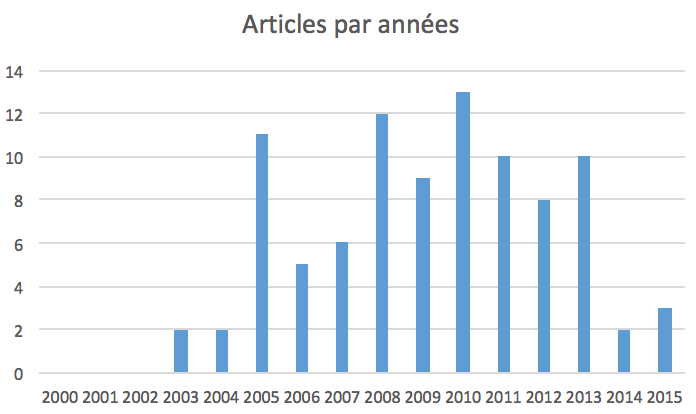
\includegraphics[scale=0.7]{articles_by_years.png}
\end{center}


\subsection{Publication Venue Distribution}
% TODO: Need a graphic for article by publishers.



\begin{center}
  \small
  \begin{tabular}{ lll }
    \bf Category & \bf Class & \bf \# of articles \\
    \hline
    \multirow{7}{*}{Detection Srategy}
    & \multicolumn{1}{l}{AI}           & \multicolumn{1}{l}{11} \\
    & \multicolumn{1}{l}{Logic}        & \multicolumn{1}{l}{22} \\
    & \multicolumn{1}{l}{Graph}        & \multicolumn{1}{l}{15} \\
    & \multicolumn{1}{l}{Metric}       & \multicolumn{1}{l}{7} \\
    & \multicolumn{1}{l}{Automata}     & \multicolumn{1}{l}{1} \\
    & \multicolumn{1}{l}{Instr./Prof.} & \multicolumn{1}{l}{10} \\
    & \multicolumn{1}{l}{Pattern Mathching}
                                       & \multicolumn{1}{l}{8} \\
    & \multicolumn{1}{l}{Others}       & \multicolumn{1}{l}{23} \\
    \hline
    \multirow{2}{*}{\textbf{Language Dependance}}
    & \multicolumn{1}{l}{Dependant}    & \multicolumn{1}{l}{XXX} \\
    & \multicolumn{1}{l}{Independant}  & \multicolumn{1}{l}{XXX} \\
    \hline
    \multirow{3}{*}{\textbf{Analysis Type}}
    & \multicolumn{1}{l}{Static}       & \multicolumn{1}{l}{XXX} \\
    & \multicolumn{1}{l}{Dynamic}      & \multicolumn{1}{l}{XXX} \\
    & \multicolumn{1}{l}{Hybrid}       & \multicolumn{1}{l}{XXX} \\
    \hline
    \multirow{3}{*}{Detection Level}
    & \multicolumn{1}{l}{Execution}    & \multicolumn{1}{l}{8} \\
    & \multicolumn{1}{l}{Source}       & \multicolumn{1}{l}{44} \\
    & \multicolumn{1}{l}{Model}        & \multicolumn{1}{l}{7} \\
    \hline
    \multirow{2}{*}{Detection generality}
    & \multicolumn{1}{l}{Specific}     & \multicolumn{1}{l}{XXX} \\
    & \multicolumn{1}{l}{General}      & \multicolumn{1}{l}{XXX} \\
    \hline
    \multirow{4}{*}{Detected Pattern Types}
    & \multicolumn{1}{l}{Creationnal}  & \multicolumn{1}{l}{23} \\
    & \multicolumn{1}{l}{Structural}   & \multicolumn{1}{l}{34} \\
    & \multicolumn{1}{l}{Behaviour}    & \multicolumn{1}{l}{49} \\
    & \multicolumn{1}{l}{Other/Not Specified}
                                       & \multicolumn{1}{l}{17} \\
    \hline
    \multirow{6}{*}{Validation Method}
    & \multicolumn{1}{l}{Benchmark}    & \multicolumn{1}{l}{7} \\
    & \multicolumn{1}{l}{Case Study}   & \multicolumn{1}{l}{40} \\
    & \multicolumn{1}{l}{Experiment}   & \multicolumn{1}{l}{8} \\
    & \multicolumn{1}{l}{Survey}       & \multicolumn{1}{l}{0} \\
    & \multicolumn{1}{l}{Other}        & \multicolumn{1}{l}{1} \\
    & \multicolumn{1}{l}{None}         & \multicolumn{1}{l}{11}
  \end{tabular}
\end{center}

\subsection{Detection Strategy}

Most of the detection strategies used fall either in the 
\textit{logic/formalisation} or \textit{other} class.
The first one was probably overly broad since it included any solution using
inference rules engines, formalisation and semantic web ontologies.
Surprisingly, the latter strategy was the focus of many articles. 


%\begin{center}
%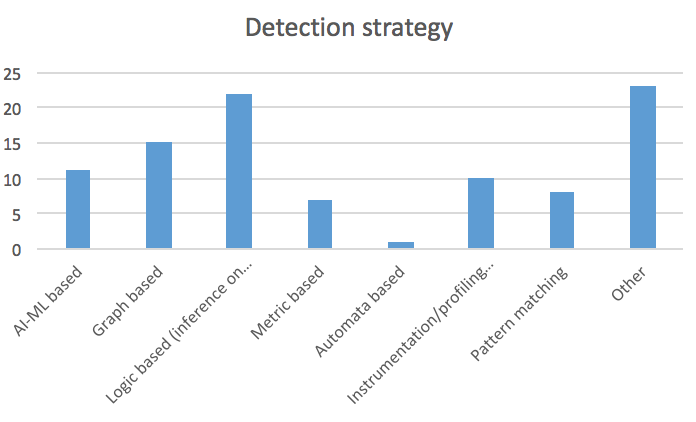
\includegraphics[scale=0.75]{detection_strategy.png}
%\end{center}


\subsection{Analysis Type}

Design pattern detection can be done either statically or dynamically.



%\begin{center}
%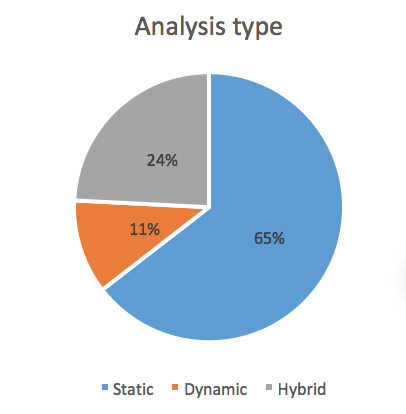
\includegraphics[scale=0.75]{analysis_type.png}
%\end{center}


\subsection{Detected Pattern Types}

The Gang of Four identified three design pattern types: creationnal,
behavioural and structural patterns.
Due to the nature of each pattern types, it is usally aknowledged that
structural patterns should be easier to detect than behavioural patterns and
that the later are easier than creationnal patterns (citation needed). 
It was expected that this ordering would appear in the number of articles
associated with each pattern types. 
However, we can see that the detection of behavioural patterns has been the
subject of more articles than the two others.

%\begin{center}
%  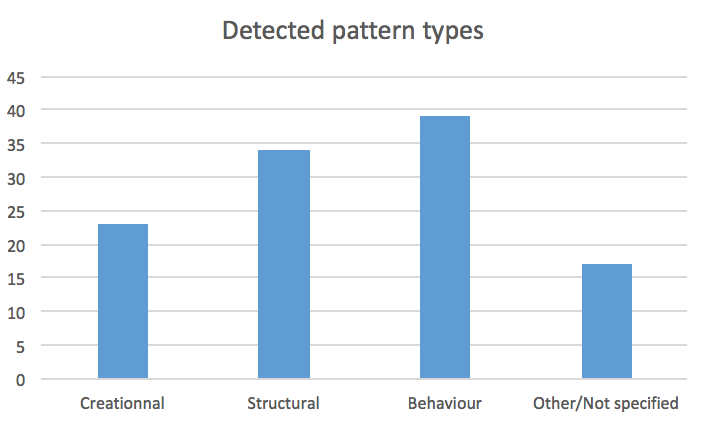
\includegraphics[scale=0.65]{pattern_types.png}
%\end{center}

This can be explained either by the fact that structural design patterns
detection is considered as an easy problem, thus less likely to be the main
focus of a research paper or by the possibility is that behavioural design
patterns are in fact easier to detect than structural ones.
However, we believe the first possibilty to be more likely.



\subsection{Language dependance}
The main focus of this category was to identify the existance of language
independant solutions to the detection of design patterns.

To identify truly generic detection methods, proposed solutions requiring a
frontend to implement have been classified as being dependant on the source
language. 

The majority of techniques are language dependant and the most used 
languages are Java and C++

But those detection methods can be easily converted to other languages
just by modifying the font-end.

Haotian and Shu[52] took a different approach by instrumenting Java bytecode

%\begin{center}
%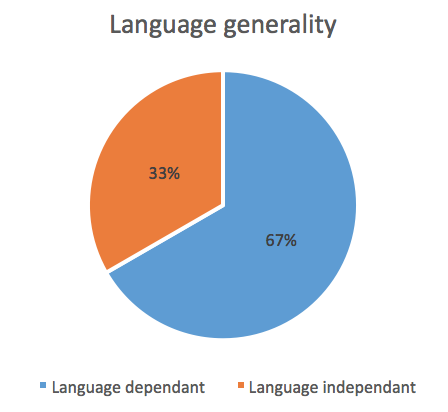
\includegraphics[scale=0.75]{language_generality.png}
%\end{center}

\subsection{Detection Level}
We found out that almost all of design patterns detection methods 
identify the patterns on a source code level, though, the detection could
be done on multiple levels.


%\begin{center}
%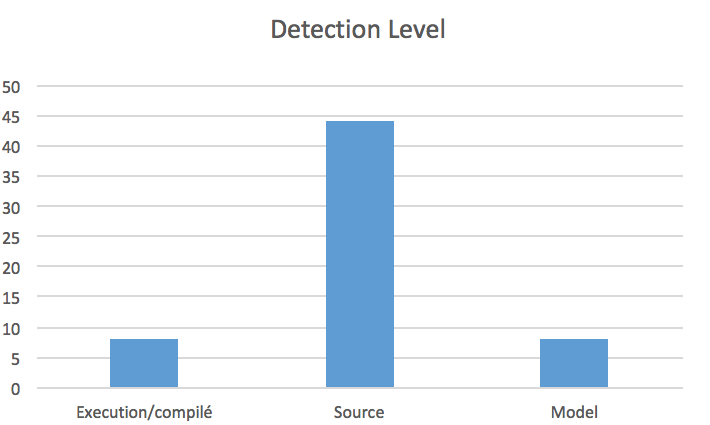
\includegraphics[scale=0.75]{detection_level.png}
%\end{center}


\subsection{Detection generality}

This category was used to expose specific pattern detection methods.
As expected, papers tend to present detection method for detecting patterns
in general.

Some papers worth noting presents specifics ways to detect particular patterns.

Marjan Heričko and Simon Beloglavec[355] presents a way of identifying
composite design pattern, composite here corresponding to the composition of
atomic DP (MVC).

Ren and Zhao[80] used and hybrid analysis based on OWL, an ontology system,
to recover instances candidates of Observer pattern followed by a dynamic
analysis to accept or reject the recovered candidates.


%\begin{center}
%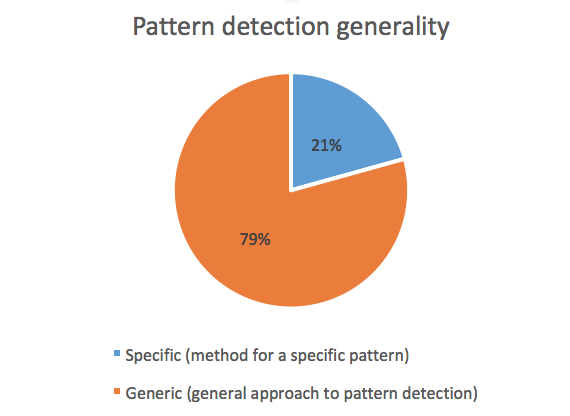
\includegraphics[scale=0.75]{detection_generality.png}
%\end{center}


\subsection{Validation Methods}

%\begin{center}
%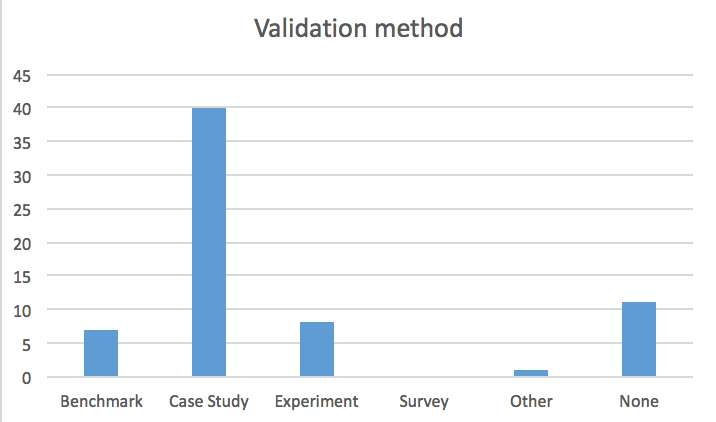
\includegraphics[scale=0.75]{validation_method.png}
%\end{center}


\subsection{Detected pattern types according to analysis type}
% Need graphics



\section{Study limitations}

\subsection{Selection Bias}

A possible limitation of our studies is the selection of a unique source for 
the articles in Scopus.
This was done to facilitate our work in the extraction of relevant articles
since Scopus offers to export the results of a search query on its database.
It has been assumed that it does an exhaustive indexing of the journals
and conferences it references and that those sources includes most of the
relevant publications that covers software design pattern detection.
To mitigate the possibility of missing relevant articles we made sure that
Scopus indexes the big venues of software engineering (ACM, Springer, IEEE, and
???).

\subsection{Screening}

There is a possibility for relevant articles to have been excluded at the
screening level due to a non representative title and abstract.
We believe the possibility to be unlikely since each article were screened by
two reviewers and that if the article had a possibly misleading title, it would
be rejected after a complete reading done before the classification phase.

As it can be seen with Cohen's kappa coefficient of the second screening group,
there were some disagreement related to the inclusion or the exclusion of some
articles.
Most of those disagreement comes from different views of what constitute a
software engineering papers and the fact that many fields have adopted the
concept of design patterns.
Even if the Cohen's kappa coefficient can be considered somewhat low for the
second group, we are confident with our screening since most disagreement have
been resolved by an experienced researcher in the field if a pair of reviewers
couldn't reach a consensus.


\subsection{Classification}

The distribution of articles between the reviewers may seem arbitrary in since it is not evenly distributed.
In fact one reviewer had two less articles to read.
This difference is due to an error when we compiled the articles that passed
the screening phase where one article was featured twice.
Since the remaining number of articles was not divisible by three, this same
reviewer had already one less article to read.
We believe this error has no effect on the overall result. \\

At first, we defined the detection level to be a disjoint classification category.
However during the classification phase of our study, we stumbled upon unfoseen cases
where the detection was done at two levels. We had to change the classification
scheme to allow those cases.



\section{Related works}



So far, no other comparable studies has been done on the field of design pattern
recognition.

(article on method validation) have identified a problem in the evaluation of design
pattern detection methods. This problem has been observed in our evaluation of the
domain in that most articles evaluates their algorithms with case studies that are
hardly comparable.




\section{CONCLUSIONS}

A conclusion section 



\addtolength{\textheight}{-12cm}   

% This command serves to balance the column lengths
                                  % on the last page of the document manually. It shortens
                                  % the textheight of the last page by a suitable amount.
                                  % This command does not take effect until the next page
                                  % so it should come on the page before the last. Make
                                  % sure that you do not shorten the textheight too much.

%%%%%%%%%%%%%%%%%%%%%%%%%%%%%%%%%%%%%%%%%%%%%%%%%%%%%%%%%%%%%%%%%%%%%%%%%%%%%%%%



%%%%%%%%%%%%%%%%%%%%%%%%%%%%%%%%%%%%%%%%%%%%%%%%%%%%%%%%%%%%%%%%%%%%%%%%%%%%%%%%



%%%%%%%%%%%%%%%%%%%%%%%%%%%%%%%%%%%%%%%%%%%%%%%%%%%%%%%%%%%%%%%%%%%%%%%%%%%%%%%%
\section*{APPENDIX}

Appendixes should appear before the acknowledgment.

\section*{ACKNOWLEDGMENT}

Acknowledgement


\begin{thebibliography}{99}

\bibitem{c1} K. Petersen, R. Feldt, S. Mujtaba, and M. Mattsson, “Systematic mapping studies in software engineering,” in Proc. of the 12th Int. Conf. on Eval. and Asses. in Soft. Eng., ser. EASE’08. Swinton, UK, UK: British Computer Society, 2008.

\bibitem{c2} www.scopus.com









\end{thebibliography}




\end{document}
